\chapter{Methodology} \label{chp:3}
%%%%%%%%%%%%%%%%%%%%%%%%%%%%%%%%%%%%%%%%%%%%%%%%%%%%%%%%%%%%%%%%%%%%%%%
In this chapter I describe the steps followed towards an automated systematic determination of flux control coefficients and disequilibrium ratios of metabolic models at steady state. 

With an entire field of data-mining established around methods of gathering knowledge from large data-sets, the metaphorical wheel did not need to be reinvented. The development of a first generation database mining-system as defined by \citeauthor{Imielinski1996, Radivojac2004, Uppalaiah2012} served as the outline to which specific methods were then developed. The overarching process of data-handling followed these four objectives.

\begin{enumerate}
\item Data processing
\item Transformation
\item Analysis
\item Visualization
\end{enumerate} 

Towards this goal, the installation of a working environment occupies the first section of this chapter. The four objectives as set forth above, will then succeed in naming subsections within which the individual components of the algorithm, as outlined in figure \ref{Algorithm}, are discussed. 

\begin{figure}[h] 
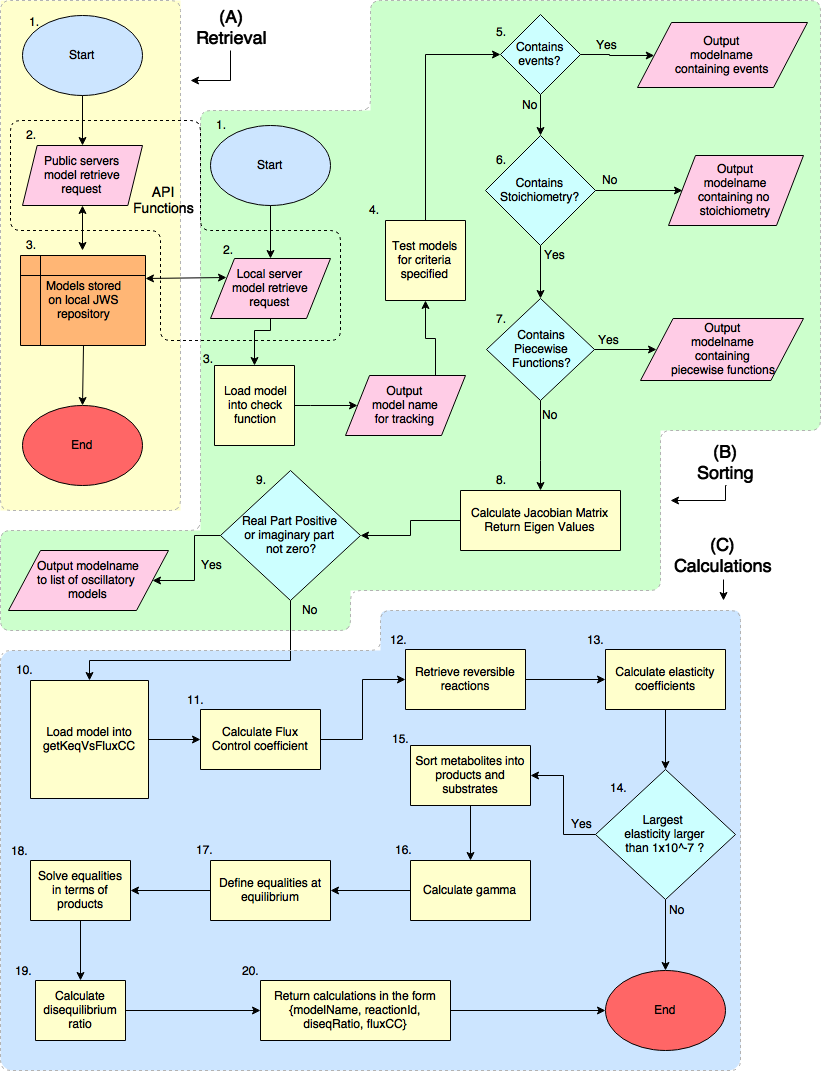
\includegraphics[width=1\textwidth]{Algorithm.png}
\centering
\caption{Overview diagram of algorithm indicating the flow of data throughout run-time. With reference to the data-handling objectives in chapter \ref{chp:3}, retrieval (A) and sorting (B) encompasses the data processing portion, whilst calculations (C) refer to the data transformation process.}
\label{Algorithm}
\end{figure}

\section{Setting up the Working environment} \label{Working Environment}
The purpose of this process was to create an isolated environment within which testing and development could occur without effecting current production systems. Another purpose of this isolation was in order to circumvent authorisation protocols which hindered the initial approach. 

The working environment was constructed in two parts; a data management component and a scripting language. For the data management component, a local instance of \href{https://jjj.bio.vu.nl}{JWSOnline}, was responsible for retrieving, storing and translating model information. Mathematica v13 functioned as the scripting environment. Mathematica was chosen as it is both the most prominent platform utilised in our laboratory as well as being specifically suited towards direct symbolic equation handling. 

The JWSOnline server instance was hosted within the Docker platform. For an even more complete JWSOnline docker installation and reference guide, please refer to the documentation available at \href{https://jws-docs.readthedocs.io/10_docker.html#building-the-jws-online-docker-image}{https://jws-docs.readthedocs.io/10_docker.html#building-the-jws-online-docker-image}.

\subsection{JWSOnline and Docker installation} \label{Docker Installation}
A locally hosted \href{https://jjj.bio.vu.nl}{JWSOnline} server was set-up, in order to achieve isolation from active production servers. This was done as to not inundate public servers with repetitive model upload, download, query and conversion operations. This proved especially useful considering the repetitive nature associated with a development and testing cycle for thousands of models. An added benefit was an observed increase in overall efficiency, taken as time to handle the entire data-set. This was due to internet connection speed and availability affecting only the initial retrieval of models from public servers. Overhead communication rates, between Mathematica and the server instance, was limited only by processor transfer rates. 

Docker is an open source platform that has the advantage of being platform agnostic. As such a Docker environment is self contained and easily reproducible. The Docker host application was downloaded and installed for the operating system in question (OSX) as instructed by the docker documentation available at \href{http://docker-sean.readthedocs.io}{http://docker-sean.readthedocs.io}. The JWSOnline Docker compose script, located at \href{http://jws-docs.readthedocs.io/10_docker.html#building-the-jws-online-docker-image}, documents the entire process of setting up JWSOnline with docker. For further documentation please refer to \href{https://docs.docker.com/compose/compose-file/#compose-file-structure-and-examples}, as a deeper description of the docker installation is outside of the scope of this thesis.

After setup, a successful installation and start up can be confirmed by visiting the local host or loop-back IP address (127.0.0.1) in the web browser of choice and being greeted by a local JWSOnline homepage.

With JWSOnline providing the model handling portion of the working environment, a communication method with the scripting language, Mathematica, was needed. The communications method native to JWSOnline, is in the form of a representational state transfer (REST) application program interface (API). As this is the basis of data transfer, the following section will provide a brief overview of example constructs, with specifics handled as applicable. 

\subsection{Communicating with JWSOnline via the \gls{rest} \gls{api}} \label{REST Communication}
A plethora of \gls{api} methods exist for various websites, but for the sake of simplicity the focus of this discussion will be on the RESTFull web service framework, as this is what is utilised by JWSOnline \cite{rest2018}.

The REST communications protocol allows applications and programs to share information with one another through a standard HTTP method. From a server perspective the \gls{rest} framework enables the control and security of access to internal application resources, while maintaining open access to services made available by such applications. These service endpoints are accessible to a client in the form of a basic URL, using the hypertext transfer protocol (HTTP), making the REST framework specifically suited towards a unified communications protocol as various applications can communicate with one another through utilizing the same protocol,irrespective of the application in question \cite{rest2018}. Case and point, the availability of the \href{http://jjj.biochem.sun.ac.za}{JWSOnline} \gls{api} enabled the interaction of the web server with other applications or scripting platforms, expanding the use of the application outside of the original project scope. 

HTTP requests can take many forms, for instance, one example can take on the following form; \href{http://jjj.biochem.sun.ac.za/rest/models/teusink/mf}{http://jjj.biochem.sun.ac.za/rest/models/teusink/mf}. In this case, linking to the mf format of the teusink model on the jjj.biochem.sun.ac.za server. Various parts of this construct were interactively altered, as described in section \ref{Data processing}, in an attempt to automate a model handling algorithm. Let us therefore build upon this request. As is indicated by the "HTTP://" portion, this request utilizes the hypertext transport protocol (HTTP) at host address \href{jjj.biochem.sun.ac.za}{jjj.biochem.sun.ac.za}. The request is directed at the \gls{rest} endpoint within the "/models" directory to return the "/teusink" model in an "/mf" format. The result returned is in the form of a javascript object no dtata pair )with the m,odeltaion (JSON name and data contents as the first and second entries respectively.

The example request can be altered to return models based on specified criteria. For example, metabolic models can be returned by altering the request construct to the following; \href{http://jjj.biochem.sun.ac.za/rest/models/?id=&organism=&process=1&jwsmodel__model_type=}{\nolinkurl{http://jjj.biochem.sun.ac.za/rest/models/?id=\&organism=\&process=1\&jwsmodel\_\_model\_type=}}. In this request, "process=1" refers to models fulfilling the prerequisite of containing metabolic processes as defined by annotations from model creation and curating strategies. A different one of these endpoints enables the integration of models from an external source to within the internal JWSOnline database. This proved useful in obtaining a larger sample size, as the \href{https://www.ebi.ac.uk/biomodels-main/}{BioModels} repository was consulted and integrated as described in section \ref{Data processing}. For more informtation on JWSOnline specific REST API endpoints, consult the JWSOnline documentation \cite{jwsdocs}. 

\section{Data processing} \label{Data processing}
Retrieval, sorting and calculations leading to data transformation will be discussed in the following section. Mirroring figure \ref{Algorithm}, The retrieval method (A) will be described first, followed by data sorting (B) and calculations (C). 

\subsection{Retrieval (A)} \label{Retrieval}
JWSOnline provides an endpoint for model retrieval from remote sources in the form of a restfull API as described above. The URL handling functions of Mathematica, namely HTTPRequest and URLExecute were used to construct a list of URLs linking to SBML models in JWSOnline as well as Biomodels. The relevant parts of the example URL construct (\href{http://jjj.bio.vu.nl/rest/fetch/?type={type}&redirect={redirect}&remote={remote}}{http://jjj.bio.vu.nl/rest/fetch/?type={type}&redirect={redirect}&remote={remote}}) was replaced by the remote model URL. This command, initiated from the local JWSOnline instance, imports and converts each model to an internal database. Folling this, the model is made available for retrieval in any of the formats supported by JWSOnline as a REST endpoint. This raised the question, which model format would be best suited for the investigation at hand?

For the development of an automated algorithm, handling metabolic model analysis, a specific model format was needed. One that proved generic enough to facilitate the development of unattended automated functions, yet flexible enough to uniformly handle differences among models from various origins, destined for a diverse range of use cases. As such five key aspects were identified as criteria for a suitable model format.

The model format had to, consistently store similar data types at the same index level. For any case where the model format does not ad-hear to a structured guideline, functions would need to be altered on a per model basis. Althou potentially possible this would prove overly complex when compared to using structured data. A native compatibility with the Mathematica V13 scripting platform was a second consideration as to model format. This consideration was termed ease of development, as functions designed by previous researchers were able to be reused. A third consideration related to the consistency of models upon format conversion. The final converted model needs to impart all of the information, without loss, that was stored within the original. The final consideration maintained that the model format of choice be directly accessible and usable from a computational perspective. In other words, a verbose linguistic format would not serve this purpose as parsing functions would need to be developed in order to utilise this data.

Since \gls{sbml} provides a standardized structure to which biological models are submitted, it seemed a logical first choice. However, although \gls{sbml} meets many of the requirements such as, predictability, accuracy and consistency, it does not meet all. Due to the fact that \gls{sbml} had no native parsing support in Mathematica at the time of development, the ease of development and accessibility aspects proved problematic. Therefore an internal JWSOnline standard, the matrix format (MF), was utilised. 

The translation process was achieved through the use of \href{https://jjj.bio.vu.nl}{JWSOnline}, whereby a \gls{sbml} model was retrieved from a remote server, converted and made available in matrix format (\gls{mf}) (One of the native JWSOnline data formats). In \gls{mf}, data is organized by content type. For example; rate-equations, metabolites, stoichiometry, parameter-sets and more are all grouped as nested lists, visually illustrated by figure \ref{fig:MatrixFormat}.  This format was chosen as it fulfilled all of the criteria as set out in list \ref{modelFormat}. It had the added advantage of enabling metabolic control calculations as discussed in section \ref{Calculations} to be done via matrix methods as described by \citeauthor{Hofmeyr2001}.

Once a model has been handled by \href{https://jjj.bio.vu.nl}{JWSOnline},the end product of the translation process is made available as an \gls{api} endpoint allowing for the retrieval of the model. For example, the Teusink model can be found at \href{https://jjj.bio.vu.nl/rest/models/teusink/mf/}{https://jjj.bio.vu.nl/rest/models/teusink/mf/}. Additional resources to JWSOnline are available at \href{http://jws-docs.readthedocs.io/8_rest.html}{JWS Docs}. 

\begin{figure}[p]
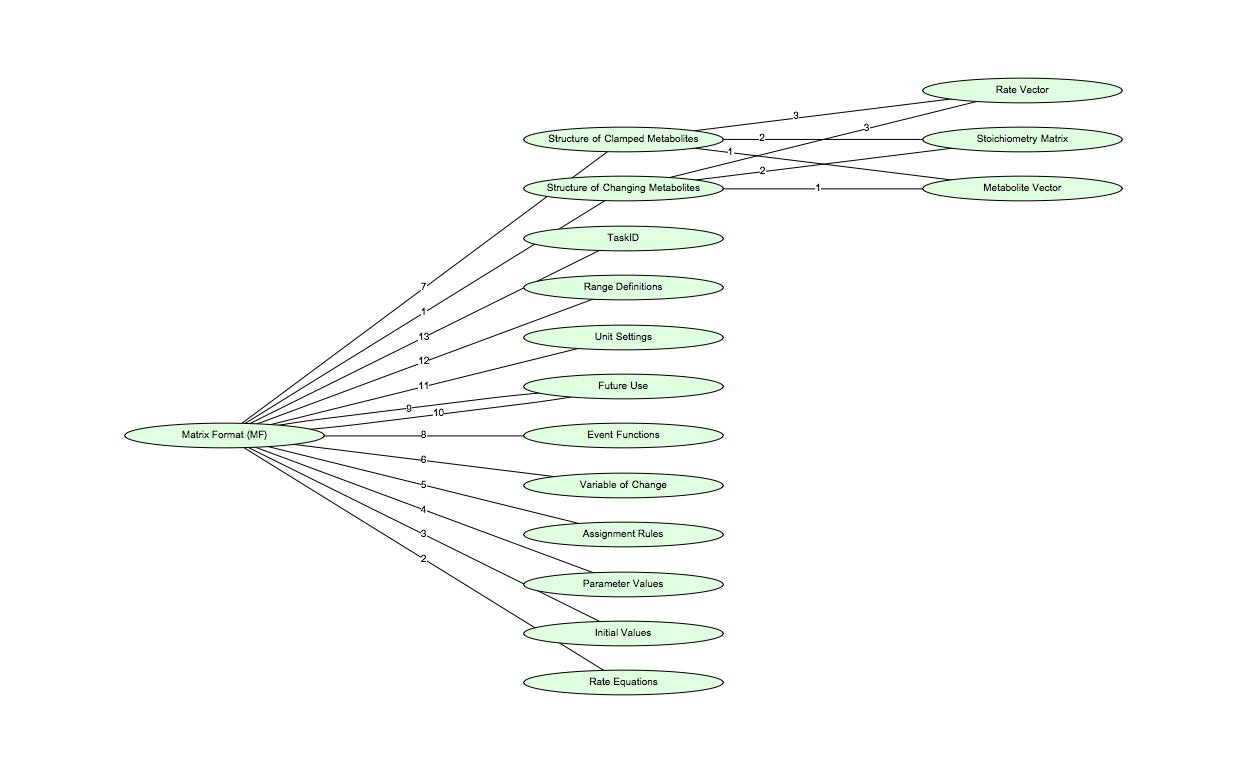
\includegraphics[width=1\textwidth]{MatrixFormat}
\centering
\caption{A graph representation of the Matrix Format (MF). Edge labels represent list index numbers and vertex labels denote content.}
\label{fig:MatrixFormat}
\end{figure}

\subsection{Sorting (B)}\label{Sorting}
Once all available models have been retrieved and stored within the local repository, the mf version was requested and returned as mentioned in section \ref{Retrieval}. These models then underwent a sorting and handling process, label B in figure \ref{fig:MatrixFormat} in order to identify where models diverge from the main algorithm (3.). This process starts off by exporting the model name to a log file. At each following sorting step, alternate log files were created, containing model names that satisfy the current conditions. Divergences in data flow was captured in these log files, that were then visualized. Vertices were defined as model names, reaction names and endpoints designated by the algorithm. Edges in turn represents relationships and direction of procedural flow. Figure \ref{fig:MatrixFormat} was the end result of visualizing these log files. This will be further discussed in section \ref{chp:4}. 

Once the initialization step was completed, a model was sent to function (4.). This function examines semantic structure as well as behaviour of models, in order to identify suitable models for the analysis at hand. The first process evaluates whether or not a model contains any event function. This is done by matching the pattern of an empty list to the appropriate sub list at index eight in the MF model (5.). A successful model is then checked for the presence of stoichiometry (6.). This is done by testing whether or not the stoichiometry list, at index one, contains any data. In other words, when the length of the list at the stoichiometry index is equal to zero, the model contains no stoichiometry and is and logged as such. Model event triggers, of the kind described above, can also be specified in terms of piece-wise functions (7.). As no a priori knowledge on the existence, timing or effect of these event triggers upon the steady state and control behaviour were available, they were also identified and logged. This identification was done based on the pattern test of a reaction containing the string term "Piecewise" as this is how the function is referred to. 

These steps served as a minimal-validation for initial models. The order of operation proved important, as these procedures were not as computationally intensive as simulation and calculation operations. Therefore computational efficiency was gained in optimizing the order of operations. 

Following the semantic and structural tests described above, the stability of a model had to be assessed. This was done by evaluating the model steady state behaviour. For this purpose the Jacobian matrix was consulted (8.). As is known from linear algebra, the eigenvalues of a Jacobian matrix holds information on the stability of a system of ODE's. The system is said to converge to a stable state where a decrease in perturbation is observed, in other words, from the Jacobian matrix, real parts of eigenvalues are negative pointing to a decrease in initial perturbations. In contrast a positive eigenvalue points to a divergence from a stable state, as a perturbation is amplified. A third condition, the occurrence of a positive eigenvalue with a non zero imaginary part, is indicative of a system oscillating around some state, be it stable or unstable periodic behaviour. As such, model names exhibiting oscillatory behaviour were identified and written to a log file. Towards a simple test of stability, a Jacobian matrix that is invertible could serve as a positive test of steady-state \cite{Hofmeyr2001}.  

A model that have reached this point in the algorithm marked a checkpoint and was written, in full MF, to a text file. Next up the model was sent for simulation and calculation procedures as is described in the following section and as can be seen in figure \ref{Algorithm} number ten.

Biological model analysis platforms range from stand-alone applications, the likes of Jarnac, COPASI, CellDesigner and BioNetGen, to  add-on modules and libraries such as LibRoadRunner, COBRA, Pysces, SimBiology and Simulink, for the Python and Matlab scripting languages respectively \cite{Sauro2000, Hoops2006, Olivier2005, Somogyi2015, Harris2016, Laurent2017}. JWSOnline, a web based interactive interface for model creation, curation and simulation was created by utilizing custom Mathematica model manipulation packages alongside a combination of the above mentioned add-on modules to python, as described by \cite{Olivier2004, jwsdocs}. The JWSOnline platform is specifically mentioned here as it formed a basis of tools, as described in section \ref{Working Environment} and \ref{Data processing}. The following section is therefore dedicated to the introduction and explanation of individual steps, leading up to the entirety of the automated model interrogation algorithm responsible for the collection of data utilized in the analysis, as is described in section \ref{Analysis}. 

\subsection{Calculations (C)} \label{Calculations}
The \gls{steady-state} of a model was calculated and the flux control coefficients were determined (10.). Internal JWSOnline functions are available in order to accomplish this task. The functions involve linear algebra methods as described by \citeauthor{Hofmeyr2001}. This method entails the reduction of a stoichiometry matrix $N$ to row echelon form by Gaussian elimination. The reduced matrix $N_R$ contains the independent reactions that can be returned to the $N$ matrix by defining a link matrix $L$ such that $N = LN_R$ \cite{Hofmeyr2001}.

Elasticity co\"efficients $\Bar{\mathcal{E}}$ is determined by taking the partial derivatives of reaction rate with respect to steady state metabolite concentrations. This notation stems from the article by \citeauthor{Hofmeyr2001} whereby the bar on $\mathcal{E}$ denotes unscaled elasticities. Scaling can be done by taking the fractional change with regards to the perturbation size. In this manner dimensionless elasticities $\mathcal{E}$ are calculated. The steady state is influenced by various parameters, populated from experimental procedures. As such, the same steady-state can occur, given differing parameters and initial start conditions.

A steady-state consists of metabolite concentrations $s$ as well as flux values $J$. Changes to these steady-state values $(s,J)$, due to perturbations of parameter $p$, can be approximated. For metabolite concentrations $s_2 = s_1 + \frac{\partial s}{\partial p}(p_2 - p_1)$ and fluxes $J_2 = J_1 + \frac{\partial J}{\partial p}(p_2 - p_1)$. 

From these  above matrices, the flux control coefficients were determined. From the product of $N_R\Bar{\mathcal{E}}L$ the Jacobian matrix $M$ is defined. Further discussions on the Jacobian matrix will follow. For now the importance lies in calculating concentration control coefficients towards the determination of flux control coefficients.

The concentration control coefficient indicates the relative changes to metabolite concentrations $s$ brought about by parameter perturbations $p$. From the matrix formalism the concentration control coefficients $\Bar{C^s}$ can be calculated from the link matrix $L$ the Jacobian matrix $M$ and the reduced stoichometry matrix $N_R$ such that $\Bar{C^s}=-LM^{-1}N_R$. Flux control coefficients were then calculated via the following equation $\Bar{C}^J = \Bar{\mathcal{E}_s}\Bar{C^s}+ I_n$ \cite{Hofmeyr2001}.

A perturbation, towards flux control co\"efficient determination, is considered as an increase in enzyme activity or concentration. Therefore a negative flux control value was deemed improbable, as an increase in enzyme concentration would logically not lead to a decrease in perturbed reaction rate. No further investigation into this was committed as it lies outside the scope of this thesis.

Considering that disequilibrium ratio calculations are only applicable within reactions proceeding in a reversible manner, a test function was developed to identify these reactions. A reversible reaction was defined as a rate equation containing a negative part within the numerator portion. This was drawn from general reaction rates where $v_{net} = v_{forward} - v_{reverse}$ thus allowing a rate to become negative (reversible) under appropriate conditions. The numerator is therefore recast into base components and tested for the presence of a negative-one term (12.). This was achieved by utilizing the tree form structures available to Mathematica leading to an equation expanded to smallest component parts. The position of these reversible reactions were then stored in a variable for use in disequilibrium calculations later. 

As can be seen from the calculations of flux control co\"efficients prior, an inverse of the Jacobian matrix is calculated (13.) \citeauthor{Hofmeyr2001}. Therefore, as the Jacobian approaches zero, an inverse would approach infinity. This introduced errors due to machine precision digit and accuracy limitations when elasticity values were too small. As such a further step in ensuring model validity was implemented via elasticity calculation checks. Maximum elasticity values of the system were compared to a threshold, chosen as $1 \cdot 10^{-10}$. The choice of this threshold was based on observation of failed calculations from models in a "trial and error manner".  Models surpassing this threshold was passed to the following step (14.). 

To calculate disequilibrium ratios, knowledge of metabolite identity (substrate/product) was needed. Metabolites were identified through the use of the stoichiometry matrix. One can extract products and substrates on the basis of stoichiometry values that are larger or smaller than zero respectively(15.). Returning a reaction id linked to product id allowed for the consistent handling of applicable reactions. In the case of multiple products only the first product was returned for use, more were not required. Once products have been identified, gamma was determined by raising each metabolite in a reaction to the power of it's corresponding stoichiometry, leading to the first part of symbolic gamma construction. From vector 
\[
S
=
\begin{bmatrix}
    s_{1} \\
    s_{2} \\
    s_{3} \\
    \vdots \\
    s_{n} 
\end{bmatrix}
\]

each component is raised to the corresponding collumn value from

\[
N 
=
\begin{bmatrix}
    x_{11} & x_{12} & x_{13} & \dots  & x_{1n} \\
    x_{21} & x_{22} & x_{23} & \dots  & x_{2n} \\
    \vdots & \vdots & \vdots & \ddots & \vdots \\
    x_{d1} & x_{d2} & x_{d3} & \dots  & x_{dn}
\end{bmatrix}
\]

leading to 

\[
S^N
=
\begin{bmatrix}
    s_1^{x_{11}} & s_2^{x_{12}} & s_3^{x_{13}} & \dots  & s_n^{x_{1n}} \\
    s_1^{x_{21}} & s_2^{x_{22}} & s_3^{x_{23}} & \dots  & s_n^{x_{2n}} \\
    \vdots & \vdots & \vdots & \ddots & \vdots \\
    s_1^{x_{d1}} & s_2^{x_{d2}} & s_3^{x_{d3}} & \dots  & s_n^{x_{dn}}
\end{bmatrix}
\]


For the second part, each of these exponents were multiplied across the respective reaction rows 

\[
V
=
\begin{bmatrix}
    V_{1} \\
    V_{2} \\
    \vdots \\
    V_{d} 
\end{bmatrix}
\]

such that

\[
\gamma 
=
\begin{bmatrix}
    s_1^{x_{11}}s_2^{x_{12}}s_3^{x_{13}} \dots s_n^{x_{1n}} \\
    s_1^{x_{21}}s_2^{x_{22}}s_3^{x_{23}} \dots s_n^{x_{2n}} \\
    \vdots\\
    s_1^{x_{d1}}s_2^{x_{d2}}s_3^{x_{d3}}\dots s_n^{x_{dn}}
\end{bmatrix}
\]

From the above it can be seen that stoichiometries of zero will result in power calculations of one. With negative and positive stoichiometries as denominators and numerators respectively, resulting in the gamma fraction \gamma of the specific reaction. $K_{eq}$ calculations where done, as an example from the Tuesink model mention earlier. The 2-Phospho-D-glycerate 2,3-phosphomutase catalyzed reaction leading from P2G to PEP is used as an example, where an equality is defined in terms of equilibrium, \textit{i.e.} the rate equation $v_n$ equals zero.

\begin{equation}
v = \frac{V_mENO([P2G] - \frac{[PEP]}{K_{eq}ENO})}{K_mENOP2G(1 + \frac{[P2G]}{K_mENOP2G} + \frac{[PEP]}{K_mENOPEP})} = 0
\end{equation}

Following this, the equality was symbolically solved in terms of the product identified in (15.). In the example case PEP is the product. As such the above equation in terms of PEP becomes

\begin{equation}\label{PEP}
PEP = K_{eq}ENOP2G
\end{equation}

From the calculations above, this reaction has

\begin{equation}\label{gamma}
\gamma=\frac{[PEP]^1}{[P2G]^1}
\end{equation}

Substitution of equation \ref{PEP} into \ref{gamma} yields $\gamma$ at equilibrium, otherwise known as $K_{eq}$. Therefore

\begin{equation}\label{Keq}
K_{eq}=K_{eq}ENO
\end{equation}

Taking equation \ref{gamma} divided by \ref{Keq} gives us the disequilibrium ratio
\begin{equation}
\rho = \frac{\gamma}{K_{eq}} = \frac{\frac{[PEP]^1}{[P2G]^1}}{K_{eq}ENO}
\end{equation}

Substituting steady-state values allows for the calculation of the numerical disequilibrium ratio. This was the generic manner in which disequilibrium calculations were done. From this methods described, two values were returned per reaction. The flux control co\"efficient as well as the disequilibrium ratio. These results were further used towards the analysis at hand.
